



Al igual que subimos en abstracción al pasar de proposiciones a predicados,
podemos plantearnos la existencia de predicados simples de más de un
argumento. A estos los solemos llamar \emph{relaciones lógicas}, aunque
también hay quien las llama \emph{correspondencias lógicas}. En particular,
a las de dos argumentos se las conoce como \emph{relaciones lógicas
binarias}.

Gracias a las relaciones lógicas binarias, podríamos representar en notación
matemática expresiones como

\begin{quote}
  El número natural elegido es menor que el número que he pensado.
\end{quote}

\noindent En esta, se hace referencia a una propiedad, ``ser menor que'',
que requiere de dos elementos para que tenga sentido. Al igual que sucedía
con los predicados de un solo argumento, esta, al particularizar para unos
valores de entrada concretos ---el valor elegido y el pensado---, tendrá un
valor lógico: verdadero o falso.

Esos elementos sin determinar se representarán, al igual que se hacía con
los predicados, como variables, que suelen tomar la forma de letras
minúsculas del alfabeto latino con tipografía en itálicas.

La relación lógica binaria se representará igual que los predicados solo que
se pondrán como subíndices dos argumentos, en lugar de uno. Así, por
ejemplo, la relación del ejemplo podría representarse como $M_{xy}$, siendo
$M$ la relación ``ser menor que'', $x$ el número natural elegido e $y$ el
pensado. Al igual que con los predicados de un argumento, también se puede
usar una notación como las de las funciones: $M(x, y)$.

Evidentemente, se tienen también relaciones lógicas de más de dos
argumentos, pero aquí nos centraremos en las de dos. Por tanto, tomaremos la
regla de asumir implícitamente que las relaciones lógicas de las que
hablamos son binarias, a menos que se especifique otra cosa.

Al contrario que con los predicados, ahora, como tenemos dos variables, los
posibles valores diferentes que podrán tomar estas conjuntamente son el
producto de los conjuntos sobre los que están definidas. Así, si $x$ se toma
de un conjunto $A$ e $y$ de uno $B$, se tendrá que para cada par $(x, y) \in
A \times B$ la relación podrá tomar un valor lógico. Sería como una
proposición, cada uno de esos casos particulares. Por ejemplo, $M_{12}= 1$
(verdadero).

Me gustaría hacer un inciso sobre los dos niveles de abstracción que estamos
usando. Muchas veces, en los textos de matemáticas, se hacen engaños que
vienen bien para la comprensión. Concretamente, me refiero a particularizar
de forma genérica. Así, en este caso, tenemos las variables $x$ e $y$ de la
relación. Podríamos hablar entonces de los valores $a$ y $b$, como si se
tratase de valores concretos, aunque en realidad no sean diferentes de los
anteriores. TKTK. A esos valores los podríamos calificar de
\emph{parámetros} (\emph{parameters}). TKTK.

\begin{example}
  Si $A = B = \{1, 2, 3\}$, la propiedad $M_{xy}$ que indica ``$x$ es
  estrictamente menor que $y$'', es una relación lógica binaria, pues, al
  particularizar $(x, y)$ en cada elemento del conjunto,

  \[ A \times B = \{(1, 1), (1, 2), (1, 3), (2, 1), (2, 2), (2, 3), (3, 1),
  (3, 2), (3, 3)\} \]

  \noindent se obtiene una proposición verdadera o falsa. Concretamente,
  será cierta para los valores $(1, 2)$, $(1, 3)$ y $(2, 3)$.
\end{example}

Dada una relación lógica binaria $R_{xy}$ sobre el producto $A \times B$, al
subconjunto $\rrel$ de $A \times B$ donde se cumple $R_{xy}$, es decir,

\[ \rrel = \{(x, y) \in A \times B \st R_{xy} \ \text{es verdadera}\} \]

\noindent se le conoce como \emph{grafo} (\emph{graph}) de la relación.
También, se podría denotar como $\text{Gr}(R_{xy})$.

\iffalse
Por cierto, tal y como acabo de hacer, en la terminología que seguiremos,
hablaremos de \emph{relaciones}, en general, y se considerará, si no se
especifica otra cosa, que se trata de relaciones lógicas binarias.
\fi

Advierta que no son lo mismo una relación lógica y su grafo, pues, en la
última se ``pierde'' la información sobre los conjuntos sobre los que se
toman los valores de las variables. Por tanto, varias relaciones lógicas
diferentes pueden contar con un mismo grafo.

Inversamente, sea $\grel$ un subconjunto de $A \times B$, $\grel \subseteq A
\times B$, definimos sobre el producto $A \times B$ la relación lógica
$P_{xy}$ que consideramos verdadera si $(x, y) \in \grel$ y false en caso
contrario.

En vista de la asociación unívoca que se puede hacer entre los subconjuntos
de $A \times B$ y las relaciones lógicas sobre $A \times B$, se define lo
siguiente.

Definición (relación binaria desde el punto de vista de la teoría de
conjuntos). Dados los conjuntos $A$ y $B$, todo subconjunto $\rrel \subseteq
A \times B$ es una \emph{relación binaria} del conjunto $A$ al conjunto $B$.

Tal y como hemos visto, los conceptos de \emph{relación lógica} y
\emph{relación conjuntista} son equivalentes, por lo que consideraremos que
son lo mismo y los denotaremos simplemente como \emph{relación}. Como
dijimos antes, si no se especifica, se considerará que se trata de una
relación binaria.

Dada una relación $\rrel \subseteq A \times B$, se denomina \semph{conjunto
inicial} de la relación $\rrel$ al conjunto $A$ y \semph{conjunto final} a
$B$.

Tal y como dijimos antes, el producto de conjuntos $A \times A$ se suele
representar por $A^2$.

Si un elemento $(x, y) \in \rrel \subseteq A \times B$, entonces se dice que
el elemento $x \in A$ está relacionado con el elemento $y \in B$ mediante la
relación $\rrel$, y se escribe $x \rrel y$, o, también, $(x, y) \in \rrel$.
Análogamente si $(x, y) \notin R$, se dice que ``$x$ no está relacionado con
$y$'' y se escribe $x \not\rrel y$.

\begin{example}
  Si tomamos $A = B = \{1, 2, 3\}$ y la relación $M_{xy}$ que indica ``$x$
  es estrictamente menor que $y$'', el grafo de esta relación es el conjunto

  \[ \rrel = \{(1, 2), (1, 3), (2, 3)\} \]

  Si $A = \{a, b\}$ y $B = \{1, 2, 3\}$, entonces $\rrel = \{(a, 2), (a,
  3)\}$ es una relación de $A$ a $B$ donde $a \rrel 2$ y $a \rrel 3$, y, sin
  embargo, $a \not\rrel 1$, $b \not\rrel 1$, $b \not\rrel 2$ y $b \not\rrel
  3$.
\end{example}

Dada una relación $\rrel$ entre $A$ y $B$, $\rrel \subseteq A \times B$, se
denomina \semph{relación inversa} (\emph{inverse relation}) de $\rrel$ a la
relación $\rrel^{-1} \subseteq B \times A$ en la que se cumple

\[ \rrel^{-1} = \{(y, x) \in B \times A \st (x, y) \in \rrel \subseteq A
\times B \} \]

\noindent Aunque esté acostumbrado a considerar que el exponente ${-1}$ es
como dividir a uno entre ese número, olvídese de eso aquí. TKTK. Más
adelante verá que esta notación tiene sentido.

\begin{example}
  Volviendo al ejemplo anterior, se tiene $\rrel^{-1} = \{(2, 1), (3, 1),
  (3, 2)\}$, en el primer caso, y, $\rrel^{-1} = \{(2, a), (3, a)\}$, en el
  segundo.
\end{example}

Dada una relación $\rrel$ entre $A$ y $B$, $\rrel \subseteq A \times B$, se
denomina \semph{conjunto original de la relación} $\rrel \subseteq A \times
B$ al siguiente subconjunto de $A$:

\[ \rrel^{-1}(B) = \{x \in A \st \exists y \in B. \ x \rrel y\} \]

\noindent \semph{conjunto imagen de la relación} $\rrel \subseteq A \times
B$, al siguiente subconjunto de $B$:

\[ \rrel(A) = \{y \in B \st \forall x \in A. \ x \rrel y\} \]

\noindent \semph{conjunto imagen del elemento $x \in A$} por la relación
$\rrel \subseteq A \times B$, a

\[ \rrel(x) = \{y \in B \st x \rrel y\} \]

\noindent y \semph{conjunto original del elemento $y \in B$} por la relación
$\rrel \subseteq A \times B$, a

\[ \rrel^{-1}(y) = \{x \in A \st x \rrel y\} \]

Muchas relaciones usuales están representadas por símbolos específicos, como
la relación ``menor o igual'', `$\leq$', en el conjunto de los números
reales, $\rset$, o la relación ``pertenece a'', `$\in$', en el ámbito de $A
\times \powset(A)$, para un conjunto cualquiera $A$, siendo $\powset(A)$ el
conjunto de las partes de $A$, es decir, el conjutno de todos sus
subconjuntos posibles.

\begin{example}
  Al considerar el conjunto de las partes de un conjunto $U$, $\powset(U)$,
  se puede considerar la inclusión de conjuntos, `$\subseteq$', como una
  relación en $\powset(U)$, es decir, se define la relación $A \subseteq B$,
  donde $A$ y $B$ son subconjuntos de $U$. Es claro que dos subconjuntos no
  vacíos tales que $A \cap B = \emptyset$ no están relacionados entre sí.
\end{example}

\begin{example}
  El conjunto

  \[ \rrel = \{(x, y) \in \rset^2 \st x - y^2 = 0\} \]

  \noindent es una relación en $\rset^2$. Al estudiar la imagen de cada
  elemento, se tiene, aislando la $y$ en la expresión en la definición del
  conjunto,

  \begin{align*}
    x - y^2 &= 0 \\
    y^2 &= x \\
    \sqrt{y^2} &= \sqrt{x} \\
    |y| &= \sqrt{x} \\
  \end{align*}

  \noindent con lo que

  \[ y = \{{-\sqrt{x}}, \sqrt{x}\} \]

  \noindent Ahora, harbá que ver los valores que se tomarían, según ciertos
  casos, pues, para algunos de los valores de $x$ no estará definida la raíz
  cuadrada. Sería

  \[
    \rrel(x) =
    \left\{
    \begin{array}{ll}
      \emptyset                 & \text{si} \ x < 0 \\
      \{0\}                     & \text{si} \ x = 0 \\
      \{{-\sqrt{x}}, \sqrt{x}\} & \text{si} \ x > 0 \\
    \end{array}
    \right.
  \]

  Por otro lado, el original de cada $y \in \rset$ es

  $$ \rrel^{-1}(y) = \{y^2\} $$

  \noindent En esta expresión es evidente que no habría que particularizar
  por casos ya que a todo elemento de $\rset$ se le puede calcular su
  cuadrado.

  Dado que $\rset^2$ se representa como un plano, entonces la relación
  $\rrel$ tiene una representación gráfica en dicho plano. Esta es la de la
  figura~\ref{fig:grafo_relacion_R}. En este caso, se trata de una parábola
  cuyo eje de simetría es el eje $OX$, con el vértice en el punto $(0, 0)$ y
  abierta hacia la derecha.

  \begin{figure}
    \centering
    \foreignlanguage{english}{
    \begin{tikzpicture}[scale=1]
      % Ejes cartesianos
      \draw[->] (-1, 0) -- (5.5, 0) node[below] {$x$};
      \draw[->] (0, -3) -- (0, 3) node[left] {$y$};

      % Representación de la relación R
      \draw[thick, domain=0:5, samples=50] plot(\x, {sqrt(\x)});
      \draw[thick, domain=0:5, samples=50] plot(\x, {-sqrt(\x)});

      % Puntos de referencia
      \filldraw (4, 2) circle (1pt);
      \filldraw (4, -2) circle (1pt);

      % Marcas de las etiquetas
      \draw (4, -0.1) -- (4, 0.1);
      \draw (-0.1, 2) -- (0.1, 2);
      \draw (-0.1, -2) -- (0.1, -2);

      % Líneas punteadas
      \draw[dashed] (4, 0) -- (4, 2) -- (0, 2);
      \draw[dashed] (4, 0) -- (4, -2) -- (0, -2);

      % Etiqueta de la relación R
      \node at (1.5, 1) {$\rrel$};

      % Etiquetas de los puntos
      \node[left] at (0, 2) {$\sqrt{x}$};
      \node[left] at (0, -2) {$-\sqrt{x}$};
      \node[anchor=north west] at (4, 0) {$x$};
    \end{tikzpicture}
    }
    \caption{Grafo de la relación $\rrel$}%
    \label{fig:grafo_relacion_R}
  \end{figure}
\end{example}

\begin{example}
  El conjunto

  \[ \grel = \{(x, y) \in \rset^2 \st x^2 + y^2 = 1\} \]

  \noindent que en el plano se representa como una circunferencia de centro
  en el punto $(0, 0)$ y radio 1, como puede ver en la
  figura~\ref{fig:grafo_relacion_G}, es una relación en $\rset$.

  Vamos a manipular la igualdad que aparece en la definición del conjunto,
  para ver si podemos aclararnos con el conjunto imagen de la relación.

\begin{align*}
  x^2 + y^2 &= 1 \\
  y^2 &= 1 - x^2 \\
  \sqrt{y^2} &= \sqrt{1 - x^2} \\
  |y| &= \sqrt{1 - x^2} \\
\end{align*}

\noindent Tenemos, entonces, que

$$
  |y| =
  \left\{
    \begin{array}{ll}
      {-\sqrt{1 - x^2}} & \ \text{si} \ \sqrt{1 - x^2} < 0 \\
      \sqrt{1 - x^2} & \ \text{si} \ \sqrt{1 - x^2} \geq 0 \\
    \end{array}
  \right.
$$

\noindent En esta expresión, nos podemos olvidar del caso $\sqrt{1 - x^2} <
0$, ya que el signo radical, si no se le antepone un signo menos, `$-$',
indica la raíz cuadrada es positiva. Por tanto, los valores de $x$ para los
que se cumpla $\sqrt{1 - x^2} < 0$ no tendrán imagen en la relación, o, lo
que es lo mismo, su imagen será $\emptyset$. Veamos cuáles son:

\begin{align*}
  \sqrt{1 - x^2} &< 0 \\
  \left(\sqrt{1 - x^2}\right)^2 &< 0^2 = 0 \\
  1 - x^2 &< 0 \\
  1 &< x^2 \\
  |x| &> 1 \\
\end{align*}

\noindent Advierta que, como el signo de raíz cuadrada indica la raíz
positiva, al elevar al cuadrado no nos preocupamos de dar la solución
positia y la negativa.

La expresión $|x| > 1$ es equivalente a la conjunción de las dos siguientes:
$x < {-1}$ y $x > 1$.

Vamos a operar ahora con la otra expresión para ver si logramos aislar a la
$x$.

\begin{align*}
  \sqrt{1 - x^2} &\geq 0 \\
  \left(\sqrt{1 - x^2}\right)^2 &\geq 0^2 = 0 \\
  1 - x^2 &\geq 0 \\
  1 &\geq x^2 \\
  |x| &\leq 1 \\
\end{align*}

\noindent Al igual que antes, al elevar al cuadrado no nos preocupamos de
dar la solución positia y la negativa.

La expresión $|x| \leq 1$ indica lo mismo que la conjunción de las dos
siguientes: $x \geq {-1}$ y $x \leq 1$. Podemos usar en este caso la forma
abreviada de la conjuncion de las dos desigualdades: ${-1} \leq x \leq 1$.

En estos casos, se tiene que $y = \pm\sqrt{1 - x^2}$, que sería lo mismo que
el conjunto con los dos elementos siguientes: $y = \{{-\sqrt{1 - x^2}},
\sqrt{1 - x^2}\}$.

% TODO No llego a ver bien por qué se toman los dos valores.

En resumen, las imágenes de la relación $\grel$, según los distintos valores
de $x$, se pueden resumir en la siguiente expresión por partes (o, por
intervalos, también se podría decir):

$$
  \grel(x) =
  \left\{
  \begin{array}{ll}
    \emptyset
      & \text{si} \ x < {-1} \ \text{o} \ x > 1 \\
    \left\{{-\sqrt{1 - x^2}}, \sqrt{1 - x^2}\right\}
      & \text{si} \ {-1} < x < 1 \\
  \end{array}
  \right.
$$

\noindent Advierta que se tiene, como particularidad, que $\grel({-1}) =
\grel(1) = \{0\}$.

Al estudiar el conjunto original de cada elemento, se tiene

$$
  \grel^{-1}(y) =
  \left\{
  \begin{array}{ll}
    \emptyset
      & \text{si} \ y < {-1} \ \text{o} \ y > 1 \\
    \left\{{-\sqrt{1 - y^2}}, \sqrt{1 - y^2}\right\}
      & \text{si} \ {-1} < y < 1 \\
  \end{array}
  \right.
$$

\noindent Como ve, es análoga al caso de la imagen. En particular, también
se tendría que $\grel^{-1}({-1}) = \grel^{-1}(1) = \{0\}$.

\begin{figure}
  \centering
  \foreignlanguage{english}{
  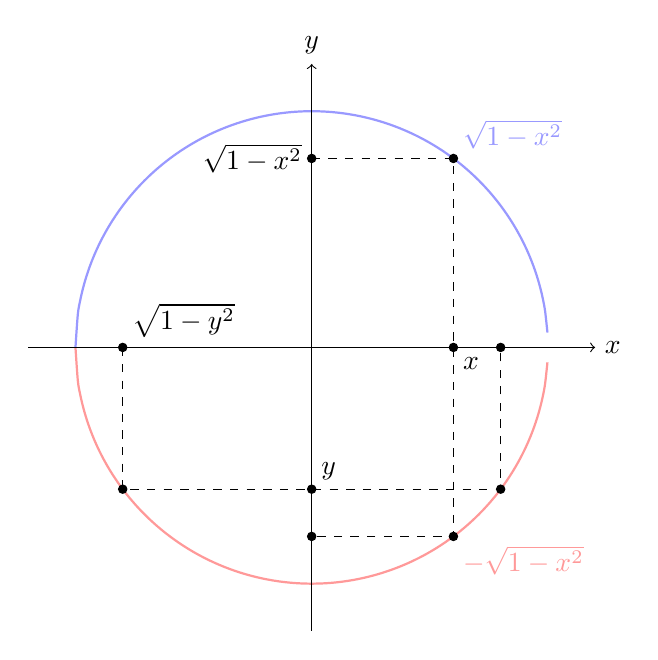
\begin{tikzpicture}[scale=3] % Ajustamos la escala para mayor claridad
    \iffalse
    % Dibujar el círculo
    \draw[thick] (0,0) circle(1); % Círculo unitario
    \fi

    % Arco de semicircunferencia superior
    \draw[thick, blue!40, domain=-1:1, smooth, samples=200, variable=\x] 
      plot (\x, {sqrt(1 - \x*\x)});

    % Arco de semicircunferencia inferior
    \draw[thick, red!40, domain=-1:1, smooth, samples=200, variable=\x] 
      plot (\x, {-sqrt(1 - \x*\x)});


    % Ejes X e Y
    \draw[->] (-1.2, 0) -- (1. 2,0) node[right] {$x$};
    \draw[->] (0, -1.2) -- (0, 1.2) node[above] {$y$};


    % Puntos principales en el círculo
    \filldraw (0.6, 0.8) circle (0.5pt);
    \filldraw (0.6, -0.8) circle (0.5pt);
    \filldraw (0.6, 0.0) circle (0.5pt) node[anchor=north west] {$x$};
    \filldraw (0, 0.8) circle (0.5pt) node[left] {$\sqrt{1 - x^2}$};
    \filldraw (0, -0.8) circle (0.5pt);
    \filldraw (0, -0.6) circle (0.5pt)
      node[anchor=south west] {$y$};
    \filldraw (-0.8, 0) circle (0.5pt)
      node[anchor=south west] {$\sqrt{1 - y^2}$};
    \filldraw (0.8, 0) circle (0.5pt);
    \filldraw (0.8, -0.6) circle (0.5pt);
    \filldraw (-0.8, -0.6) circle (0.5pt);

    % Líneas punteadas para las proyecciones
    \draw[dashed] (0, 0.8) -- (0.6, 0.8) -- (0.6, -0.8) -- (0, -0.8);
    \draw[dashed] (-0.8, 0) -- (-0.8, -0.6) -- (0.8, -0.6) -- (0.8, 0);

    % Etiquetas de los puntos
    \node[blue!40, above right] at (0.6, 0.8) {$\sqrt{1-x^2}$};
    \node[red!40, below right] at (0.6, -0.8) {$-\sqrt{1-x^2}$};

    % Etiqueta del círculo
    \node[above left] at (-0.7, 0.7) {$\grel$};
  \end{tikzpicture}
}
  \caption{Grafo de la relación $G$}%
  \label{fig:grafo_relacion_G}
\end{figure}
\end{example}

\begin{example}
  En el conjunto producto del ejemplo TKTK, se considera la relación de
  ganadores

  \[ \grel = \{(A, g), (A, p), (B, d), (C, j)\} \]

  \noindent cuya representación gráfica dentro del conjunto producto $J
  \times P$, o grafo de la relación $\grel$ está en la
  figura~\ref{fig:ejercicio-juego-2}, aunque también puede representarse en
  términos de diagramas de flechas como en la
  figura~\ref{fig:diagrama-flechas-g}.

  \begin{figure}
    \centering
    \foreignlanguage{english}{
    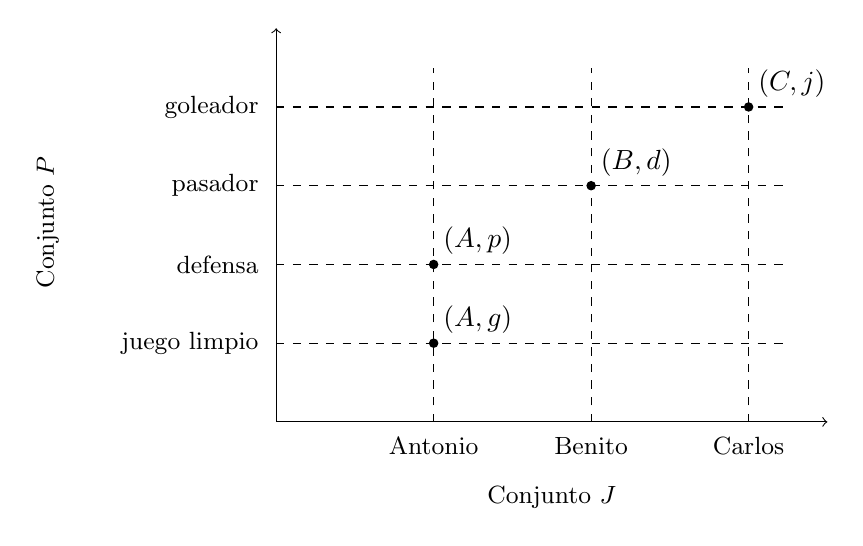
\begin{tikzpicture}[scale=1]
      % Ejes
      \draw[->] (0,0) -- (7,0);
      \draw[->] (0,0) -- (0,5);

      % Etiquetas de los ejes
      \node[left, rotate=90] at (-2.9, 3.5) {\small Conjunto $P$};
      \node[below] at (3.5, -0.7) {\small Conjunto $J$};

      % Etiquetas en los ejes
      \node at (2, -0.3) {\small Antonio};
      \node at (4, -0.3) {\small Benito};
      \node at (6, -0.3) {\small Carlos};

      \node[left] at (-0.1, 1) {\small juego limpio};
      \node[left] at (-0.1, 2) {\small defensa};
      \node[left] at (-0.1, 3) {\small pasador};
      \node[left] at (-0.1, 4) {\small goleador};

      % Líneas punteadas horizontales
      \foreach \y in {1,2,3,4} {
          \draw[dashed] (0,\y) -- (6.5,\y);
      }

      % Líneas punteadas verticales
      \foreach \x in {2,4,6} {
          \draw[dashed] (\x,0) -- (\x,4.5);
      }

      % Puntos y etiquetas
      \filldraw (2, 1) circle (1.5pt) node[anchor=south west] {$(A, g)$};
      \filldraw (2, 2) circle (1.5pt) node[anchor=south west] {$(A, p)$};
      \filldraw (4, 3) circle (1.5pt) node[anchor=south west] {$(B, d)$};
      \filldraw (6, 4) circle (1.5pt) node[anchor=south west] {$(C, j)$};
    \end{tikzpicture}
    }
    \caption{Representación de la relación $\grel$ entre $J \times P$}
    \label{fig:ejercicio-juego-2}
  \end{figure}

  \begin{figure}
    \centering
    \foreignlanguage{english}{
    \begin{tikzpicture}
      % Nodos de los conjuntos como óvalos
      \node[draw, ellipse, minimum width=2cm, minimum height=4cm] (J)
        at (0, 0) {};
      \node[draw, ellipse, minimum width=2cm, minimum height=4cm] (P)
        at (4, 0) {};

      % Etiquetas de los conjuntos
      \node (J) at (0, 2.2) {$J$};
      \node (P) at (4, 2.2) {$P$};

      % Etiqueta de la relación
      \node at (2, 2.5) {$\rrel$};

      % Elementos en J
      \node[fill, circle, inner sep=1pt] (A) at (0, 0.3)
        [label=left:$A$] {};
      \node[fill, circle, inner sep=1pt] (B) at (0, 1.4)
        [label=left:$B$] {};
      \node[fill, circle, inner sep=1pt] (C) at (0, -1.2)
        [label=left:$C$] {};

      % Elementos en P
      \node[fill, circle, inner sep=1pt] (p) at (4, 1.2)
        [label=right:$p$] {};
      \node[fill, circle, inner sep=1pt] (j) at (4, 0.4)
        [label=right:$j$] {};
      \node[fill, circle, inner sep=1pt] (d) at (4, -0.4)
        [label=right:$d$] {};
      \node[fill, circle, inner sep=1pt] (g) at (4, -1.2)
        [label=right:$g$] {};

      % Conexiones (relación G)
      \draw[dashed] (A) -- (p);
      \draw[dashed] (A) -- (g);
      \draw[dashed] (B) -- (d);
      \draw[dashed] (C) -- (j);
      \draw[->, thick] (J) -- (P);
    \end{tikzpicture}
    }
    \caption{Diagrama de la relación $G$ entre $J$ y $P$}
    \label{fig:diagrama-flechas-g}
  \end{figure}

  Además, se tiene que el conjunto imagen de cada jugador es

  \begin{center}
    \begin{tabular}{lcr}
    $\grel(A) = \{g, p\}$
      & $\grel(B) = \{d\}$
      & $\grel(C) = \{j\}$ \\
  \end{tabular}
  \end{center}

  \noindent y que el conjunto origen de cada premio es

  \begin{center}
  \begin{tabular}{lccr}
    $\grel^{-1}(g) = \{A\}$
      & $\grel^{-1}(p) = \{A\}$
      & $\grel^{-1}(d) = \{B\}$
      & $\grel^{-1}(j) = \{C\}$ \\
  \end{tabular}
  \end{center}
\end{example}

Como es evidente, para la relación $\rrel \subseteq A \times B$ el conjunto
$\powset(A \times B)$ será el conjunto de todas las relaciones posibles en
$A \times B$. En consecuencia, toda relación puede darse por extensión o por
comprensión. TKTK.

Definición (composición de relaciones). Dadas las relaciónes

\begin{align*}
  \rrel \subseteq A \times B \\
  \srel \subseteq B \times C \\
\end{align*}

\noindent se define una relación entre los conjuntos $A$ y $C$, denominada
\emph{composición} de las relaciones $\rrel$ y $\srel$, que denotamos por
$\srel \circ \rrel \subseteq A \times C$, como

$$ \srel \circ \rrel = \{(x, y) \in A \times C \st \exists y \in B \quad
\text{tal que} \ x \rrel y \ \text{e} \ y \srel z\} $$

En realidad, el concepto de composición de relaciones puede ser más amplio
que el que hemos dado aquí. Si se fija, se podría haber referido, de forma
más general, a las relaciones

\begin{align*}
  \rrel \subseteq A \times B \\
  \srel \subseteq C \times D \\
\end{align*}

TKTK

Lógica relacional. Esta lógica es similar a la lógica de predicados, pero
empleando relaciones lógicas simples como ``palabras básicas''. Se emplean
las mismas reglas sintácticas y conectivas, y los mismos cuantificadores que
en la lógica de predicados, si bien en este caso se puede utilizar un
cuantificador para cada argumento.

El uso de cuantificadores satisface el principio siguiente: Toda relación
$R_{xy}$ definida sobre el producto cartesiano $A \times B$ de dos conjuntos
$A$ y $B$ y precedida por un cuantificador por cada variable, como, por
ejemplo,

\[ \forall x \in A \ \forall y \in B. \ R_{xy}, \quad \exists x \in A \
\forall y \in B. \ R_{xy} \quad \text{o} \quad \forall y \in B \ \exists x
\in A. \ R_{xy} \]

\noindent es una proposición en el sentido de que se le puede atribuir sin
ambigüedad el valor verdadero o falso. Cuando no haya duda sobre los
conjuntos $A$ y $B$, se escribirá simplemente

\[ \forall x \ \forall y \ R_{xy}, \quad \exists x \ \forall y \ R_{xy}
\quad \text{o} \quad \forall y \ \exists x \ R_{xy} \]

\begin{example}
  Si se tiene una relación $P_{xy}$ donde $A = \{a, b, c\}$ y $B = \{1,
  2\}$, entonces $\forall x \ \forall y \ P_{xy}$ es la proposición

  \[ P_{a1} \land P_{a2} \land P_{b1} \land P_{b2} \land P_{c1} \land P_{c2}
  \]

  La proposición $\forall x \ \exists y \ P_{xy}$ es la proposición

  \[ (P_{a1} \lor P_{a2}) \land (P_{b1} \lor P_{b2}) \land (P_{c1} \lor
  P_{c2}) \]

  \noindent mientras que in intercambio en el orden de los cuantificadores,
  $\exists y \ \forall x \ P_{xy}$, conduce a la proposición

  \[ (P_{a1} \land P_{b1} \land P_{c1}) \lor (P_{a2} \land P_{b2} \land
  P_{c2}) \]

  \noindent que no es equivalente a la anterior pues si $\rrel = \{(a, 1),
  (b, 2), (c, 1)\}$ entonces $\forall x \ \exists y \ P_{xy}$ es verdadera
  mientras que $\exists y \ \forall x \ P_{xy}$ es falsa.

  La proposición $\exists x \ \forall y \ P_{xy}$ toma el valor de la
  proposición

  \[ (P_{a1} \land P_{a2}) \lor (P_{b1} \land P_{b2}) \lor (P_{c1} \land
  P_{c2}) \]

  \noindent mientras que la proposición $\forall y \ \exists x \ P_{xy}$ es

  \[ (P_{a1} \lor P_{b1} \lor P_{c1}) \land (P_{a2} \lor P_{b2} \lor P_{c2})
  \]

  \noindent y $\exists x \ \exists y \ P_{xy}$ toma el valor de la propiedad

  \[ P_{a1} \lor P_{a2} \lor P_{b1} \lor P_{b2} \lor P_{c1} \lor P_{c2} \]
\end{example}

\begin{example}
  En el ejemplo anterior, hemos comprobado que cuando los cuantificadores
  son distintos el orden de colocación de los mismos altera el valor lógico
  de la proposición. Analicemos otro ejemplo: la proposición

  \[ \forall x \in \rset \ \exists n \in \nset. \ n > x \]

  \noindent significa que para cada número real existe un número natural que
  lo supera, cosa que es cierta. Concretamente, a esta propiedad se la conoce
  como la Propiedad Arquimediana de $\rset$, y la veremos en un captítulo
  posterior. Un simple cambio de orden en los cuantificadores conduce a

  \[ \exists n \in \nset \ \forall x \in \rset. \ n > x \]

  \noindent que significa que existe un número natural que supera a todos los
  números reales, cosa que sabemos que es falsa.
\end{example}

\begin{example}
  Para negar una proposición con varios cuantificadores, se procede de la
  manera siguiente. Por ejemplo, busquemos la negación de $\exists x \in A \
  \forall y \in B. \ P_{xy}$, que escribimos como $\exists x \ \forall y \
  P_{xy}$ ya que se sobrentiende que se conocen esos conjuntos.

  \begin{align*}
    \neg(\exists x \ \forall y. \ P_{xy})
      &\iff \forall x \ \neg(\forall y. \ P_{xy}) \\
      &\iff \forall x \ \exists y. \ \neg P_{xy} \\
  \end{align*}
\end{example}

Definición. Relación homogénea. Se dice que una relación es
\semph{homogénea} cuando se define sobre un producto de conjuntos iguales,
es decir, cualquier relación $\rrel \subseteq U \times U$, para un conjunto
$U$ cualquiera.








